\providecommand{\main}{..}
\documentclass[\main/master.tex]{subfiles}
\begin{document}
\chapter{Presentation}\label{chp:example-1}




\subsection{Cavendish Experiment}
Torsion Pendulum is an oscillator made of mass hung by a string from a fixed point so it could swing free. The Cavendish experiment, first performed in the 17th century, measures the gravitational force between masses using a torsional pendulum.
\par 
Assuming no friction or other damping force (simple harmonic oscillator) when a mass is interduced, there are two sources of torque in the system; restoring tourqe by wire torsion and by gravitational force. At equilibrium, tourqes are canceled out at an angle $\theta$.

\begin{figure}[htbp]
	\centering
	\fbox{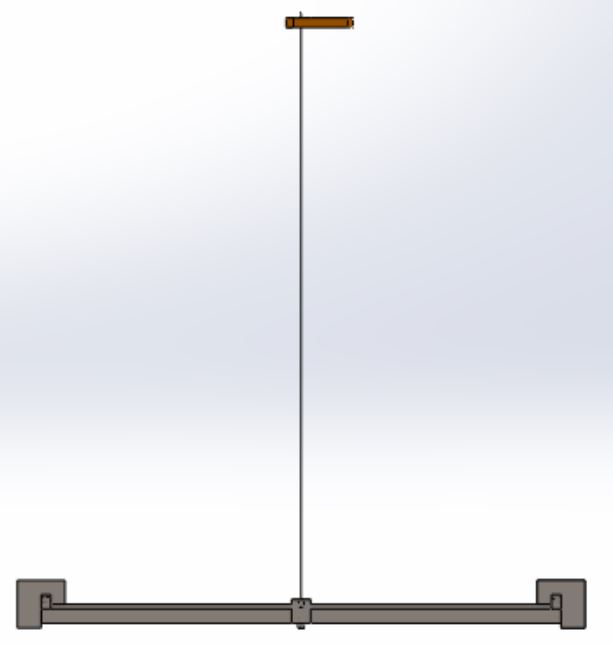
\includegraphics[scale=1.2]{\main/images/2 - theoretical background/torsion_pendulum.JPG}}
	\caption[pendulum]{the torsion pendulum}
	\label{fig:torsion_pendulum}
\end{figure}
\begin{equation}
\overrightarrow{\tau} = \kappa\theta = LF = L\frac{GmM}{r^2}    \label{eqn:gravitation_tourqe}
\end{equation}
\newpage

\subsection{System Noises}
Pendulum is placed inside vacuum reducing brownian motion, acoustic waves and friction, vacuum chamber is reducing magnetic noise as a faraday cage. Also  at vacuum brownian motion from envirement coupling is reduced.
\par
The quantum uncertainty due to brownian motion is the main noise source. The quantum uncertainty at a given temperture (assuming above basic energy level).
\begin{equation}
\delta\theta = \sqrt{\frac{KT}{\kappa}}\propto{T}  \label{eqn:radiation force}
\end{equation}
\begin{equation}
\delta\theta(t) = \delta\theta cos(\omega_0 t)   \label{eqn:pid_error}
\end{equation}
The noise reductance enables to damp and cool the pendulum temperture. Damping is made using a PID feedback loop. Having an effective lower temperature would enable measuring smaller angles enlarging the SNR and the measuremnt sensetivity.
\begin{figure}[htbp]
	\centering
	\fbox{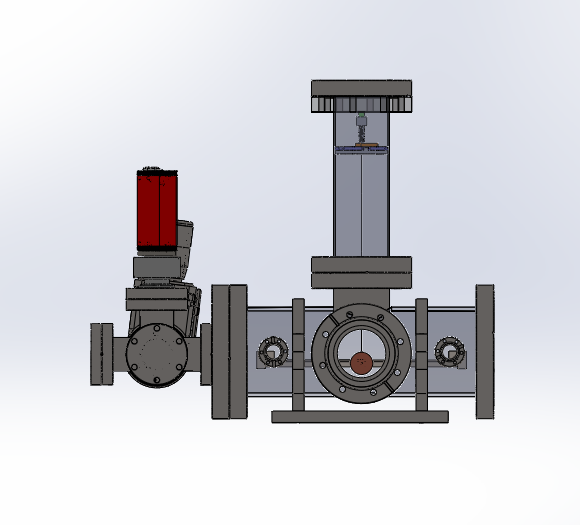
\includegraphics[scale=0.7]{\main/images/4 - methods and results/total_chamber.png}}
	\caption[total]{the total chamber}
	\label{fig:total}
\end{figure}

\newpage
\subsection{PID Controller}
proportional–integral–derivative controller (PID controller) is a feedback based control system, used for time continuouse control of a process, so output would be close to set point.
\par
Controller continuously calculates error from set point, and applies external correction based on a proportional $P$, integral $I$ and derivative $D$ gain to error. The control is having three tuning parameters to correction; $K_P, K_I, K_D$. The response (control variable) is a weighted sum of the control terms.


\begin{figure}[htbp]
	\centering
	\fbox{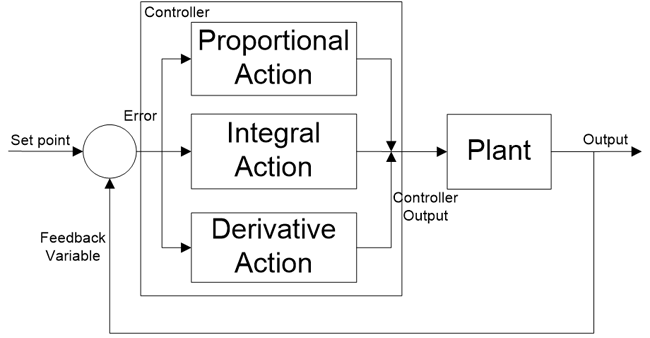
\includegraphics[scale=0.3]{\main/images/2 - theoretical background/PID.png}}
	\caption[PID]{PID controller feedback loop; from wikipedia}
	\label{fig:PID_scheme}
\end{figure}
\begin{equation}
u(t) = K_Pe(t)+K_I\int_{0}^{t}e(t)+K_D\frac{de(t)}{dt}   \label{eqn:PID_eq}
\end{equation}

P is proportional to the current error, I is proportional to past error value's integration, D is proportional to error current change rate (future).
\par
Optimal control is achieved by balancing the responses,depending on the characteristics of the specific process. 


\newpage
\subsection{Radiation Pressure Force}
The PID external correction tourqe is by two modulation controlled LED sources. The light is causing radiation pressure on the pendulum.
\par
Fast modulated light source with high intensity cause a small controlled force. The diffrence between two light sources from both ends of pendulum adds a controled small damping tourqe. 
\begin{equation}
F = \frac{2\eta\Theta}{{c}} \label{eqn:radiation force}
\end{equation}
\begin{equation}
\tau\approx d\Delta F = \frac{2d}{{c}} (\eta_1\Theta_1 -\eta_2\Theta_2) \label{eqn:radiation tourqe}
\end{equation}
The radiation pressure tourqe assuming light fields direction perpendicular to surface, $\Theta$ is the light source radiant flux [watt], and $\eta$ is the coupling efficiency. The center of mass distance from rotation axis $d$ of both forces is even.
\par
The setup could produce very small tourqes; light sources of 1 watt maximum power and 8bit modulation steps could produce nano-$N\cdot m$ to pico-$N\cdot m$ tourqes. 

\newpage
\subsection{Radiation pressure}

Radiation pressure is pressure on the surface due to momentum exchange with electromagnetic field, including momentum of light. The pressure is causing force on the surface, although the force is usually insignificant.  
\par
The radiation pressure force depends on the angle of surface compare to electromagnetic field, surface intesity reflectance and absorbance, and the power of light hitting the surface $\Theta_i$ (radiant flux, measured in watts). There is coupling efficiency $\eta$ due to the light losses while passing through light transmitters (such as light guide or fiber), and size difference between the light beam size and the target size. The incident radiation pressure, when $\alpha$ is the field angle compare to surface area $A$, and $c$ the speed of light. As a first approximation assume that the beam is focused tightly enough that variation over the surface are negligible. 
\begin{equation}
P_{incident} = \frac{\frac{\Theta_i}{A}cos^2(\alpha)}{c} = \frac{\eta\cdot \Theta_{source}\cdot cos^2(\alpha)}{{A\cdot c}} \label{eqn:radiation_pressure}
\end{equation}
The radiation pressure assuming light field direction perpendicular to surface and angle neglected. 
\begin{equation}
P_{incident} = \frac{\eta\Theta_{source}}{{Ac}} \label{eqn:radiation_pressure_perpendicular}
\end{equation}

The radiation force assuming surface is a reflective material.
\begin{equation}
F = P_{total}\cdot A = (P_{incident}+P_{emitted})\cdot A = P_{incident}(1+R)A \label{eqn:radiation_force}
\end{equation}
\begin{equation}
F \approx 2P_{incident}A = \frac{2\eta\Theta_{source}}{{c}}\cdot \frac{A}{A} \label{eqn:radiation_force_reflective}
\end{equation}
\begin{equation}
F = \frac{2\eta\Theta_{source}}{{c}} \label{eqn:radiation_force_power}
\end{equation}




\newpage
\subsection{System Design}
The pendulum angle displacement is measured with a front mirror. Chamber build is  with two small viewports on the sides, used by the PID system to damp noises, one in front of the pendulum's mirror. 
\par
Measurement is made when valve closed and engine off, to prevent rotation noise.
\begin{figure}[htbp]
	\centering
	\fbox{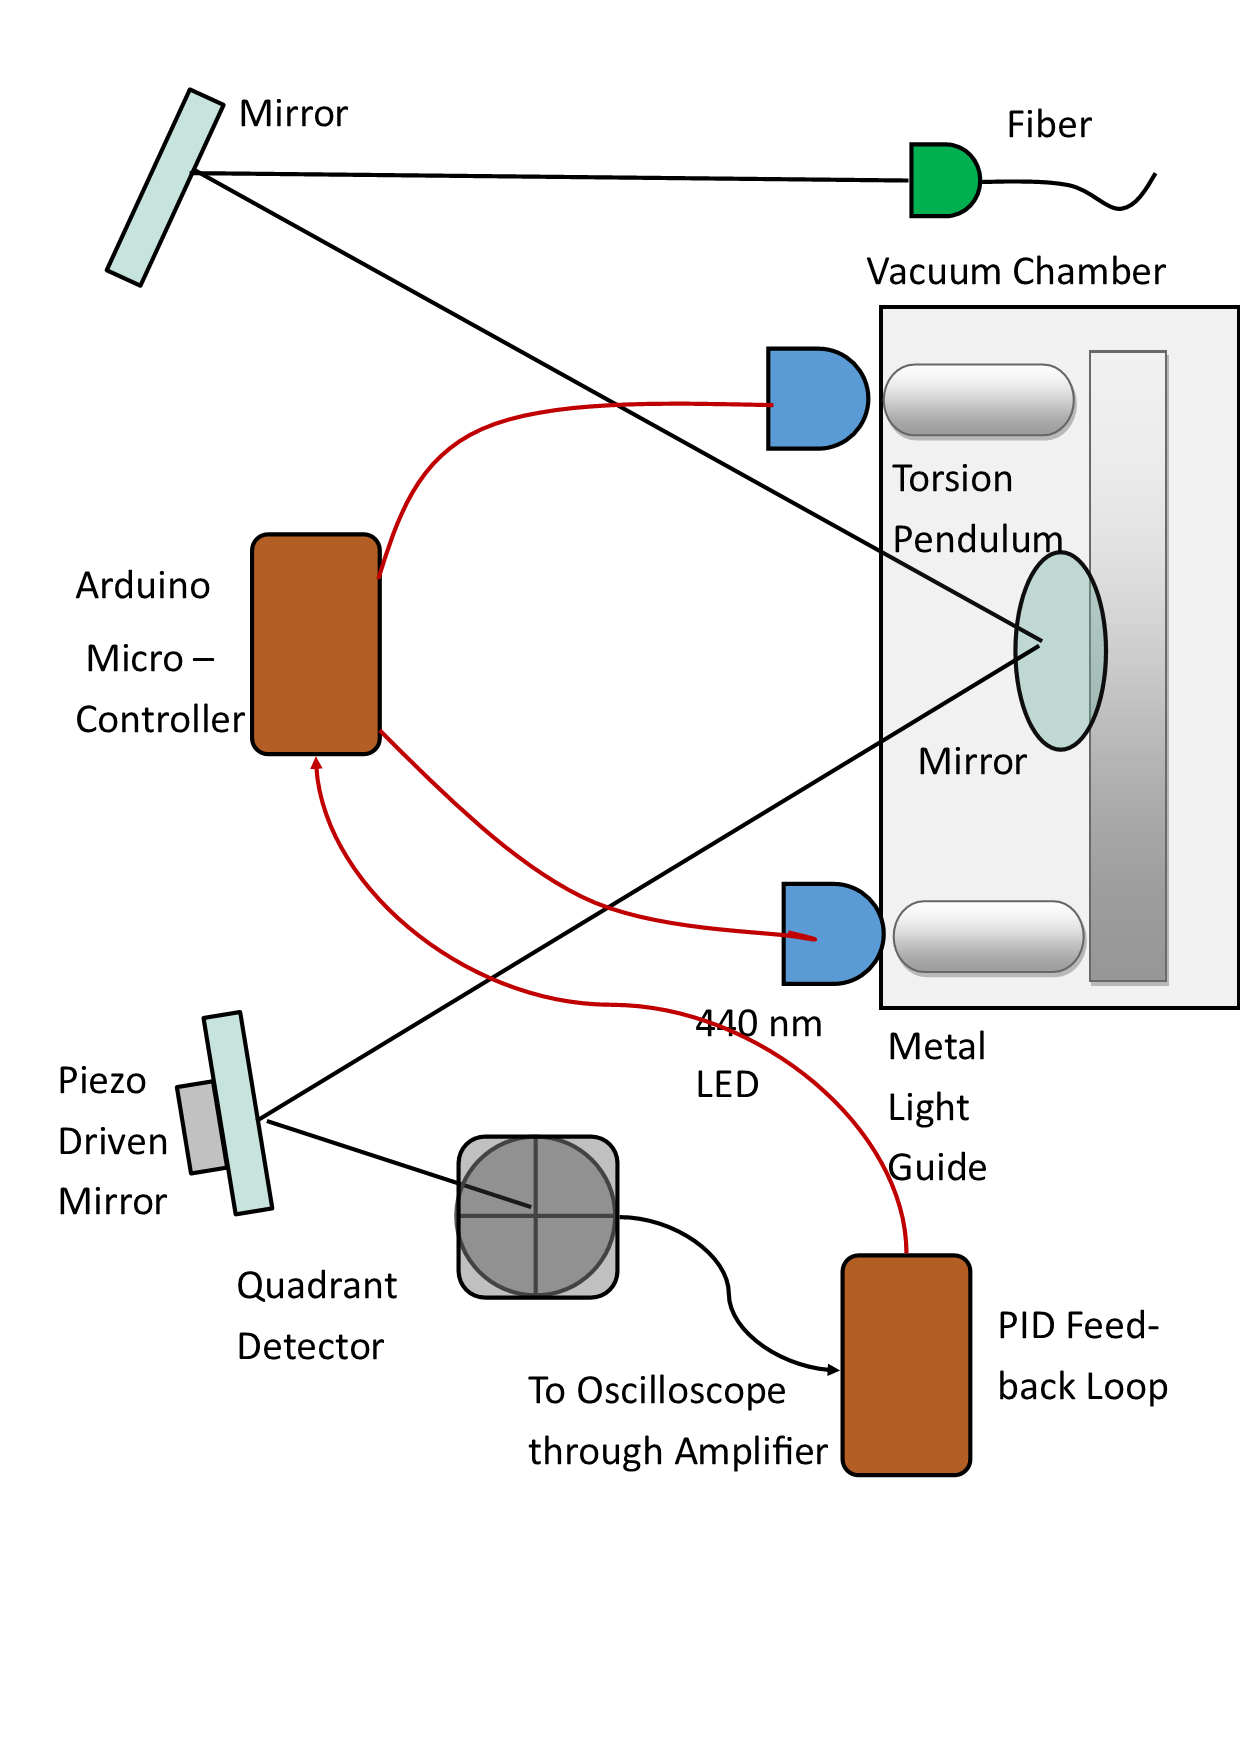
\includegraphics[scale=0.3]{\main/images/4 - methods and results/setup.png}}
	\caption[optical setup]{the optical setup}
	\label{fig:optical setup}
\end{figure}

\newpage

\subsubsection{Simple Harmonic Oscillator}

\begin{equation}
\tau = -\kappa\cdot\theta  = I\cdot\ddot{\theta}   \label{eqn:undamped_motion_equation}
\end{equation}
\begin{equation}
\theta(t) = \theta_{max}cos(\omega_0 t )    \label{eqn:undamped_motion_equation}
\end{equation}
\begin{equation}
\omega_0  = \frac{2\pi}{T} = \sqrt{\frac{\kappa}{I}}   \label{eqn:undamped_motion_equation}
\end{equation}
The natural resonant frequency $\omega_0$ and time period of oscillation $T$ are determined by the physical constants of the pendulum.


\subsubsection{Damped Oscillator}
If the system is also having damping (friction) which is proportional to the velocity, the system is a damped oscillator.

\begin{equation}
\tau = -\kappa\cdot\theta - b\dot{\theta}  = I\cdot\ddot{\theta}   \label{eqn:damped_motion_equation}
\end{equation} 
\begin{equation}
\ddot{\theta} + 2\xi\omega_0\dot{\theta} + \omega_0^2\theta = 0   \label{eqn:damped_motion_equation}
\end{equation}
\begin{equation}
\theta(t) = Ae^{-\frac{t}{\tau}\cdot(1+\sqrt{1-\frac{1}{\xi^2}})} + Be^{-\frac{t}{\tau}\cdot(1-\sqrt{1-\frac{1}{\xi^2}})}    \label{eqn:damped_motion_equation}
\end{equation}
\begin{equation}
\tau = \frac{1}{\xi\omega_0} = \frac{1}{\frac{b}{2\sqrt{I\kappa}}\sqrt{\frac{\kappa}{I}} }= \frac{2I}{b}  \label{eqn:damping_time}
\end{equation}
The system damping ratio $\xi$ is the ratio between critical damping and the actual damping, determining the damping type and time $\tau$ of system. Sytem could either be undamped, overdamped, critically damped or underdamped.
\begin{figure}[htbp]
	\centering
	\fbox{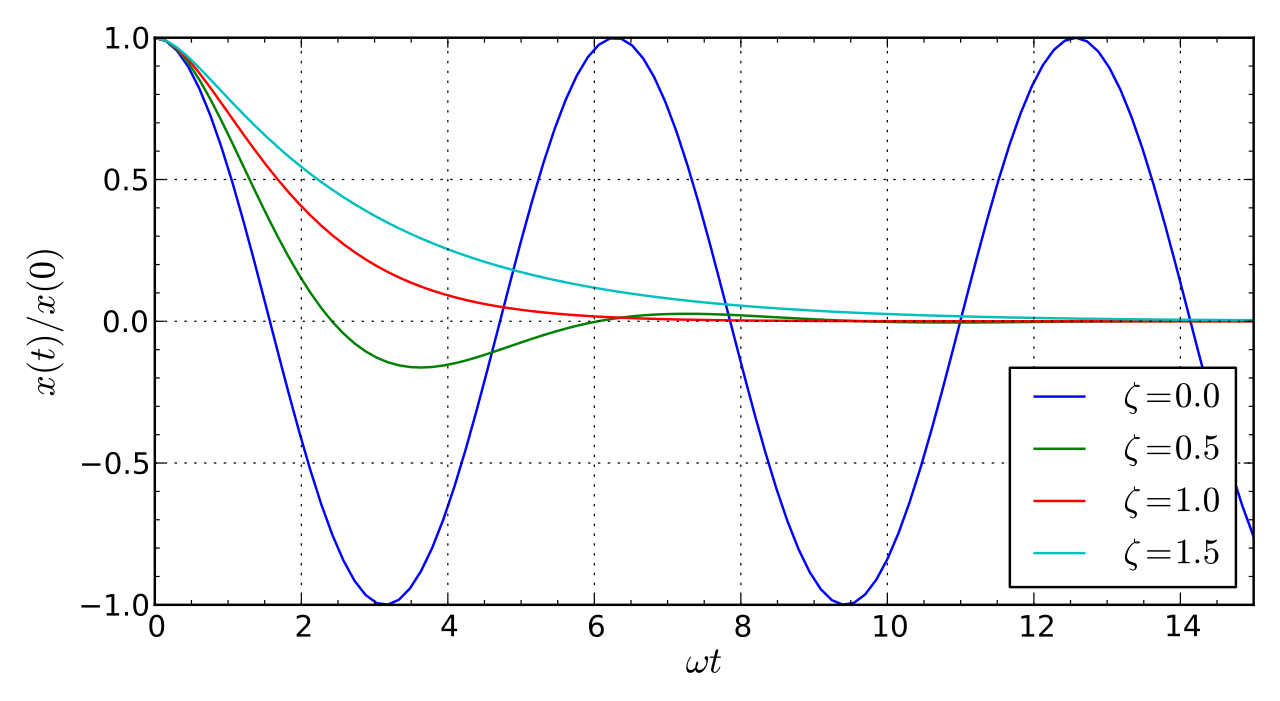
\includegraphics[scale=0.2]{\main/images/2 - theoretical background/damping.png}}
	\caption[damped]{damped oscillators; from wikipedia}
	\label{fig:damped_oscillators}
\end{figure}

\newpage
\subsubsection{Damped Oscillator}

Overdamped ($\xi > 1$); due to high friction, the system cannot oscillate and decays exponentialy to equilibrium position. 
\begin{equation}
\theta(t) = Ae^{-\frac{t}{\tau}\cdot(1+\sqrt{1-\frac{1}{\xi^2}})} + Be^{-\frac{t}{\tau}\cdot(1-\sqrt{1-\frac{1}{\xi^2}})}    \label{eqn:overdamped_motion_equation}
\end{equation}
Critically damped ($\xi = 1$); due to high friction, the system cannot oscillate and decays exponentialy to equilibrium position. For a fixed $I, \kappa$, choosing $b$ to be at the critical damping value gives
the fastest return to equilibrium position. Although there is overshoot this is often a desirable property.

\begin{equation}
\theta(t) = \theta_{max}\cdot e^{-\frac{t}{\tau}}     \label{eqn:underdamped_motion_equation}
\end{equation}
 underdamped ($\xi < 1$); amplitude decreases in time due to the friction while oscillating with a lower frequency due to the damping. When the damping coefficient is small enough, the frequency change is neglected.
\begin{equation}
\theta(t) = \theta_{max}\cdot e^{-\frac{t}{\tau}}cos(\sqrt{1-\xi^2}\omega_0 t ) =  \theta_{max}\cdot e^{-\frac{t}{\tau}}cos(\omega t )    \label{eqn:underdamped_motion_equation}
\end{equation}

\subsubsection{Driven Oscillator}
If the damped oscillator system is further affected by an external time-dependent tourqe $\tau(t)$,  the system is called driven oscillator.
\begin{equation}
\tau(t) -\kappa\cdot\theta - b\dot{\theta}  = I\cdot\ddot{\theta}   \label{eqn:driven_motion_equation}
\end{equation} 
\begin{equation}
\ddot{\theta} + 2\xi\omega_0\dot{\theta} + \omega_0^2\theta = \frac{\tau(t)}{I}   \label{eqn:damped_motion_equation}
\end{equation}

\newpage
\subsection{PID}
The PID acts as friction, gradually working when the ossicilations are at the maximum speed to slow them down, and remove the tourqe energy.
\par
If the defined set point is zero, the error is the measured variable. When PID tuned correct damped pendulum is at critical damping and ossiclations become smaller. PID error is getting samller and damping response becomes small. 


\begin{equation}
e(t) = \theta(t) = \theta   \label{eqn:error}
\end{equation}
\begin{equation}
\tau_{PID} = -\gamma\cdot\dot{\theta}   \label{eqn:friction_tourqe}
\end{equation}
The sytem is a damped oscillator, with an external force correction, which inserts tourqe to the oscillator.
\begin{equation}
\kappa\cdot\theta - \gamma\cdot\dot{\theta}  + I\cdot\ddot{\theta} = 0   \label{eqn:damped__pid_motion_equation}
\end{equation}
\begin{equation}
\gamma\dot{\theta}  = Fr   \label{eqn:damped__pid_motion_equation}
\end{equation}
\begin{equation}
\dot{\theta} = \omega_0\theta_{max}sin(\omega_0 t )    \label{eqn:undamped_motion_equation}
\end{equation}
\begin{equation}
\dot{\theta}_{max} = \omega_0\theta_{max} = \theta_{max}\cdot\frac{2\pi}{T}    \label{eqn:undamped_motion_equation}
\end{equation}
\begin{equation}
\gamma  = \frac{F_{max}r}{\dot{\theta}_{max}} =\frac{F_{max}rT}{\theta_{max}2\pi}    \label{eqn:damped_pid_motion_equation}
\end{equation}
\begin{equation}
\tau =  \frac{2I}{\gamma}  \label{eqn:damping_time}
\end{equation}
The PID damping $\gamma$ and damping time $\tau$ depends on the initial oscillations angle. If the angle is too large compare to the inserted force, the system is extremly underdamped and the PID affect is neglected. The damping time would be infinite and the system would keep on ossicilating.


\newpage
\subsubsection{Overshoot}
Overshoot is when output signal or function exceeds the target value. The response signal is not accurate compare to target. In control theory there are two wanted conflicting properties; an accurate response (small overshoot), and small risetime (fast response). 

\begin{equation}
PO = 100\cdot e ^{\frac{-\xi\pi}{\sqrt{1-\xi^2}}} = \frac{output-target}{target}   \label{eqn:percentage_overshoot}
\end{equation}
\subsubsection{Control Stability}
Using PID control does not guarantee optimal control or stability. Well tuned control would a reach the desired set point fast and accurate, and keep over time.
\par
The controller response is its response to error. When controller gains are too high, instead of critical damping there is overdamping causing overshoot, due to the high gain the overshoot response overshoots to the other side, causing the system to be driven.



\subsubsection{Phase delay}
When there is a phase delay between mesurement and response (due to noise filtering for example).
\begin{equation}
e(t) = \theta(t) = \theta_{max}cos(\omega_0 [t-t_0] ) = \theta_{max}[ cos(\omega_0 t)cos(\omega_0 t_0) - sin(\omega_0 t)sin(\omega_0 t_0)]    \label{eqn:error}
\end{equation}
Causing pid tourqe to be a time dependent, and having a driven oscilator. 
\begin{equation}
\tau_{PID}(t) = -\gamma\cdot\dot{\theta}(t)   \label{eqn:friction_tourqe}
\end{equation}
\begin{equation}
\ddot{\theta} + 2\xi\omega_0\dot{\theta} + \omega_0^2\theta = \frac{\tau(t)}{I}   \label{eqn:damped_motion_equation}
\end{equation}
Since a damped oscilator frequency is getting smaller the affect becomes more dominant as the pendulum is damped. The closer $t_0$ to zero the driving could be neglected (tourqe is less time dependent). We try to prevent that with as close to real time sampling as possible, with fast 8ms delay sampling using arduino controller. Also we limit the PID response to work only at regions where response doesn't have to be as accuurate, not at the peaks when pendulum doesn't move. 

\begin{figure}[htbp]
	\centering
	\fbox{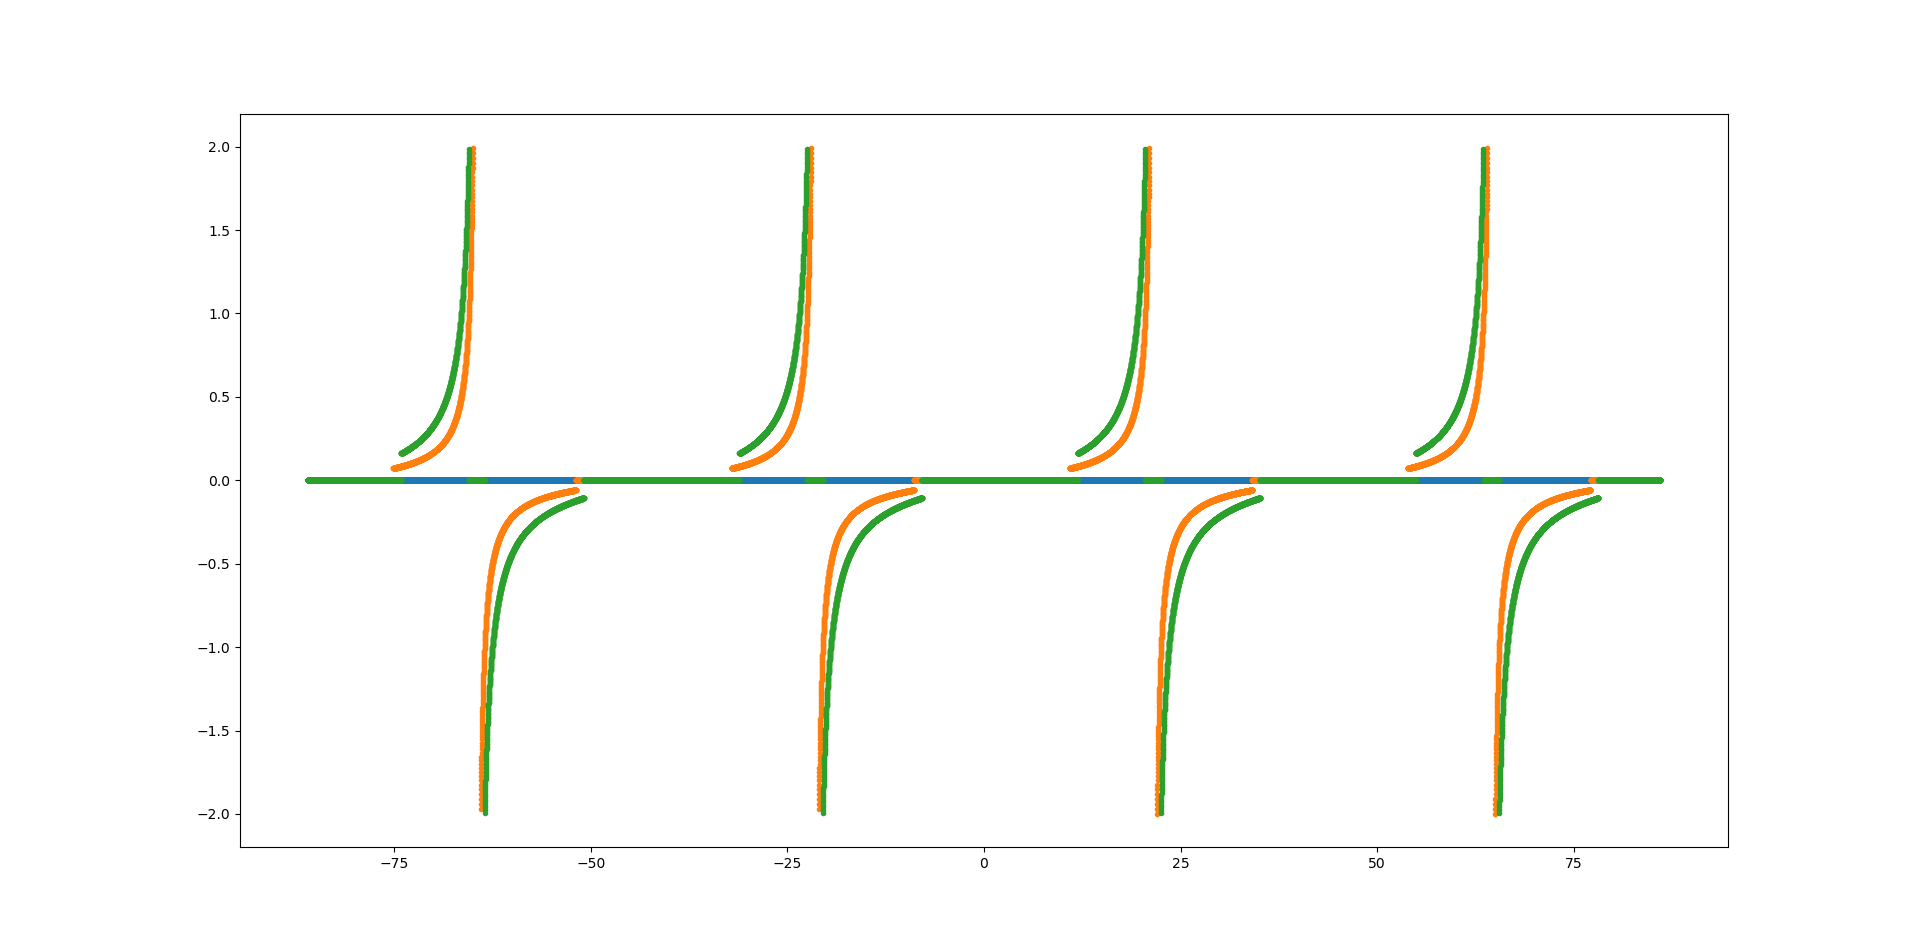
\includegraphics[scale=0.2]{\main/images/4 - methods and results/phase.png}}
	\caption[phase delay]{phase delay comparison}
	\label{fig:phase delay}
\end{figure}
\newpage
\subsubsection{Results}











\end{document}